 \section{The Ramsey-Cass-Koopmans model}\label{ramsey-model}
 
 \subsubsection{Assumptions}
\begin{itemize}
    \item Large number of identical firms, each having access to the production function $F(K,AL)$;
    \item Workers and capital are in competitive factor markets, implying they are paid the respective marginal productivity's;
    \item $A$ is given and grows at rate $g$;
    \item As firms are owned by households all profits accrue to them. 
\end{itemize}

\subsubsection{Consumption in the Ramsey Model}

In the Solow Model the consumption was given by an exogenous function. 

\begin{itemize}
    \item $ \bar{H}$ = The total number of households
    \item $ \frac{L(t)}{\bar{H}} $ = Workers per household
\end{itemize}
In continuous time, we have the following maximization problem: 

\begin{equation}
\begin{aligned}
& \underset{x(t)}{\max}
& & \int_{t=0}^{\infty} \rho ^{-\eta t}.V[x(t);S(t)].dt \\
& \text{subject to}
& & \dot{S}(t)= g\left[x(t);S(t)\right]\\
\label{tab:ramsey1}
\end{aligned}
\end{equation}

In discrete time we have the following: 

\begin{equation*}
\begin{aligned}
& \underset{x(t)}{\max}
& &   \sum_{t=0}^{\infty} (1+\eta)^{-t}.V(x_{t};S_{t}) \\
& \text{subject to} 
& & \Delta S_{t+1}=S_{t+1}-S_{t}=g(x_{t},S_{t}) \\ 
& \text{Where}
& & \eta \in (0,1)
\end{aligned}
\end{equation*}

Where $V(t)$ is the Utility Flow, or the Felicity Function which is defined as:

\begin{equation}
    V(t)=u(t)*\frac{L(t)}{\bar{H}}
\end{equation}


\begin{equation}
    u(t)=\frac{C(t)^{1-\theta}-1}{1-\theta} , \theta>0  
\end{equation}

$C(t)$ is the consumption of each household member. 
Considering $L(t)=L(0).e^{nt}=>L(t)=e^{nt}$ because $L(0)=1$. 
Thus we can rewrite \ref{tab:ramsey1} as follows: 

\begin{equation}
\begin{aligned}
 & \underset{U}{\max}
 & & \int_{t=0}^{\infty} e^{(-\rho-\theta.n) t}*\frac{C(t)^{1-\theta}-\rho^{(1-\theta).n.t}}{1-\theta}dt \\
 & \text{subject to} 
 & & \dot{k}(t)=w(t).L(t) + R(t).K(t)-c(t)-\delta K(t) 
\end{aligned}
\end{equation}

The constraint in this case implies that profits are zero. That is because the model assumes competitive markets. 

\paragraph{}

By optimizing through an Hamiltonian we get

\begin{equation*}
    H=\frac{C(t)^{1-\theta}-e^{(1-\theta).n.t}}{1-\theta}+\lambda.(w.L+R.K-c-\delta .K)
\end{equation*}

From this Hamiltonian function we get the optimization conditions, from which we take some conclusions and important functions for the model. 

From the first order condition for K comes: 

\begin{equation}
    \frac{\partial H}{\partial K}=\lambda.(r-\delta)=-\dot{\lambda}+\eta.\lambda \implies \frac{\dot{c}}{c}=\frac{1}{\theta}[(R-\delta)-(\rho - \theta.n)]
\label{tab:euler1}
\end{equation}

This result is very important for this model, and the Diamond model, as it translates the consumption dynamics in the Economy. This is known as the Euler Consumption Function.

From the first order condition for C comes: 

\begin{equation}
\begin{aligned}
& & \frac{ \partial H}{\partial C}=C^{(-\theta)}-\lambda=0 \\
&  \text{because} 
& \lambda=C^{-\theta}
\end{aligned}
\end{equation}

From the first order condition for $\lambda$ comes 

\begin{equation}
    \frac{ \partial H}{ \partial \lambda}=w.L + r.K - c - \delta.K=\dot{K}
\end{equation}

\subsubsection{Variables in the intensive form}
Now rewriting \ref{tab:euler1} in the intensive form:

\begin{equation}
    \frac{\dot{c}}{c}=\frac{f'(k)-(\delta + \rho + \theta.g)}{\theta}
    \label{tab:euler intensive}
\end{equation}

All other variables in the intensive form are like the ones for the Solow model. 

\subsubsection{Consumption dynamics}

We know that a steady state $\dot{c}=0$. Hence, the following condition must apply: 

\begin{equation*}
\begin{aligned}
    f'(k^*)=\rho + \delta + \theta.g \iff\\
 \iff f'(k^*)=\rho + n - n + g - g + \delta + \theta . g \iff \\
  \iff  f'(k)=(n+g+\delta)+[\rho - n - (1-\theta).g]
\end{aligned}
\end{equation*}
\paragraph{}

We know that $(n+g+\delta)$ is equal to $f'(k_{G})$ by the golden rule of capital accumulation and we know that $[\rho - n - (1-\theta).g]$ is positive. Hence, we can infer that $f'(k^*)>f'(k_{G})$ and so $k^*<k_{G}$, demonstrating that there can be no dynamic inefficiency in a Ramsey Economy.

\subsubsection{Capital dynamics}
Capital in the Ramsey model works very much like in the Solow model. It's only worth noting this: 

\begin{equation*}
\begin{aligned}
    \dot{K}=w.L+R.K-C-\delta . K \implies \\
    \implies \dot{k}=f(k)-c-(n+g+\delta)k
\end{aligned}
\end{equation*}

\subsubsection{Steady States}
Any steady state in the Ramsey Model has to comply to the following condition:

\begin{equation*}
    \lim_{t\rightarrow \infty}e^{-(\rho - \theta .n)t}.c(t)^{-\theta}.K(t)=0
\end{equation*}

\subsubsection{System Dynamics}



\begin{equation*}
\begin{aligned}
    \begin{cases} \dot{c}=c.\frac{f'(k)-\delta-\rho-\theta .g}{\theta} \\ 
    \dot{k}=f(k)-(n+g+\delta )k-c
    \end{cases}
\ \implies
\begin{cases}
     \dot{c} \simeq    \frac{f'(k^{*})-\delta-\rho-\theta . g}{\theta}.(c-c^{*})+c^{*}.\frac{1}{\theta}.f''(k^{*}).(k-k^{*}) \\
     \dot{k} \simeq [f'(k^{*}-(n+g+\delta)].(k-k^{*})-(c-c^{*})
\end{cases}
\end{aligned}
\end{equation*}

\paragraph{}
To put in matrix form,

$$    
\begin{bmatrix}
    \dot{c} \\ 
    \dot{k}
\end{bmatrix}
=
\begin{bmatrix}
    0 &  \frac{c^{*}}{\theta}.f''(k^{*}\\
    -1 & f'(k^{*})-(n+g+ \delta)
\end{bmatrix}
.
\begin{bmatrix}
    (c-c^{*}) \\
    (k-k^{*})
\end{bmatrix}
$$

Let 
$
\begin{bmatrix}
    0 &  \frac{c^{*}}{\theta}.f''(k^{*}\\
    -1 & f'(k^{*})-(n+g+ \delta)
\end{bmatrix}$
= $J^{*}$, we can see, then, 

\begin{itemize}
    \item $det(J^{*})=\frac{c^{*}}{\theta}.f''(k^{*})= \lambda_{1}.\lambda_{2} <0$
    \item $tr(J^{*})=f'(k^{*})-(n+g+\delta)=\lambda_{1}+\lambda_{2} >0$
\end{itemize}

From this we can take the equilibrium dynamics, as a graph: 

\begin{figure}[H]
    \centering
    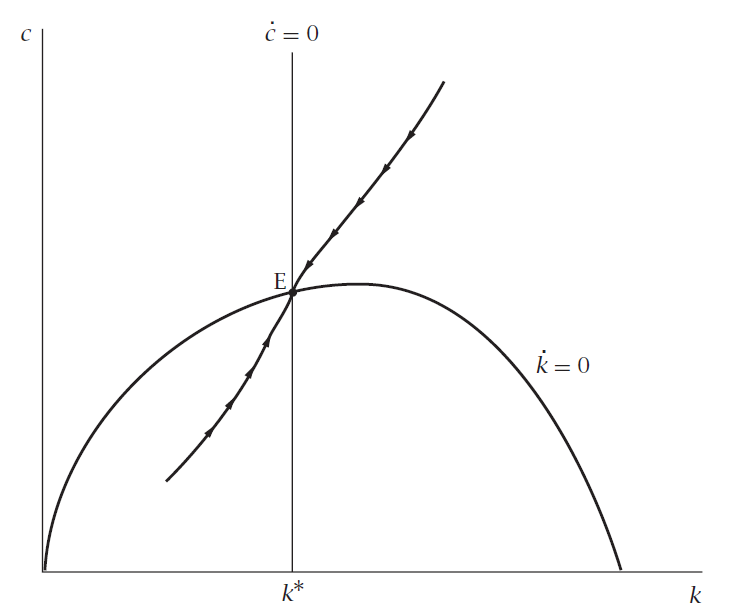
\includegraphics[width=.7\textwidth]{Ramsey.PNG}
    \caption{Ramsey Model Dynamics}
    \label{fig:my_label}
\end{figure}

We can see there is only one stable equilibrium, given by point E, whose equilibrium path we can see by the contract curve. 

The initial point of the economy in terms of consumption and capital accumulation is very important on this model, as it may change the results entirely. 
    \begin{itemize}
        \item If the starting point is between the contract curve and the capital path, it will converge to the contract curve. This will happen on points to the right of E, as well as to the left. 
        \item If the starting point is below the capital accumulation path, to the right of the contract curve, the economy will accumulate capital infinitely, until it reaches a point of zero consumption. This will violate the transversality condition.
        \item If the starting point is above the capital accumulation path, to the left of E, the economy will increase consumption and decrease capital accumulation until it reaches a point of zero capital. This violates the condition $\rho>n+(1-\theta)g$.
        \item We should also note that there is an equilibrium at (0,0), but it is unstable, as a little increase in capital will increase consumption, and this will start a cycle of more consumption - more capital which will end at the stable growth path of the contract curve and eventually point E.
        \item Furthermore the maximum point of the capital accumulation curve $\dot{k}=0$ gives us the golden rule level of capital accumulation, after which increasing capital will only decrease consumption. 
    \end{itemize}

\subsubsection{Fiscal Policy and the government}
For simplicity we'll assume government will take a lump sum tax $T$ (this achieves the same results, without increasing the difficulty of the math if it were a distortionary tax) to finance it's consumption, $G$. Thus equations in the model change as such: 

\begin{equation*}
    \dot{K}=w.L+R.K-T-c-\delta \implies Y=C+I+G
\end{equation*}
We should note that $w.l+R.K=Y$, and $T=G$, which makes government expenditure in this model have a negative impact on total output, by having a negative impact on total capital. 


\paragraph{}
Also,
\begin{equation*}
    \dot{k}=f(k)-c-\gamma-(n+g+\delta).k
\end{equation*}
Where $\gamma=\frac{G}{AL}$

\begin{figure}[H]
    \centering
    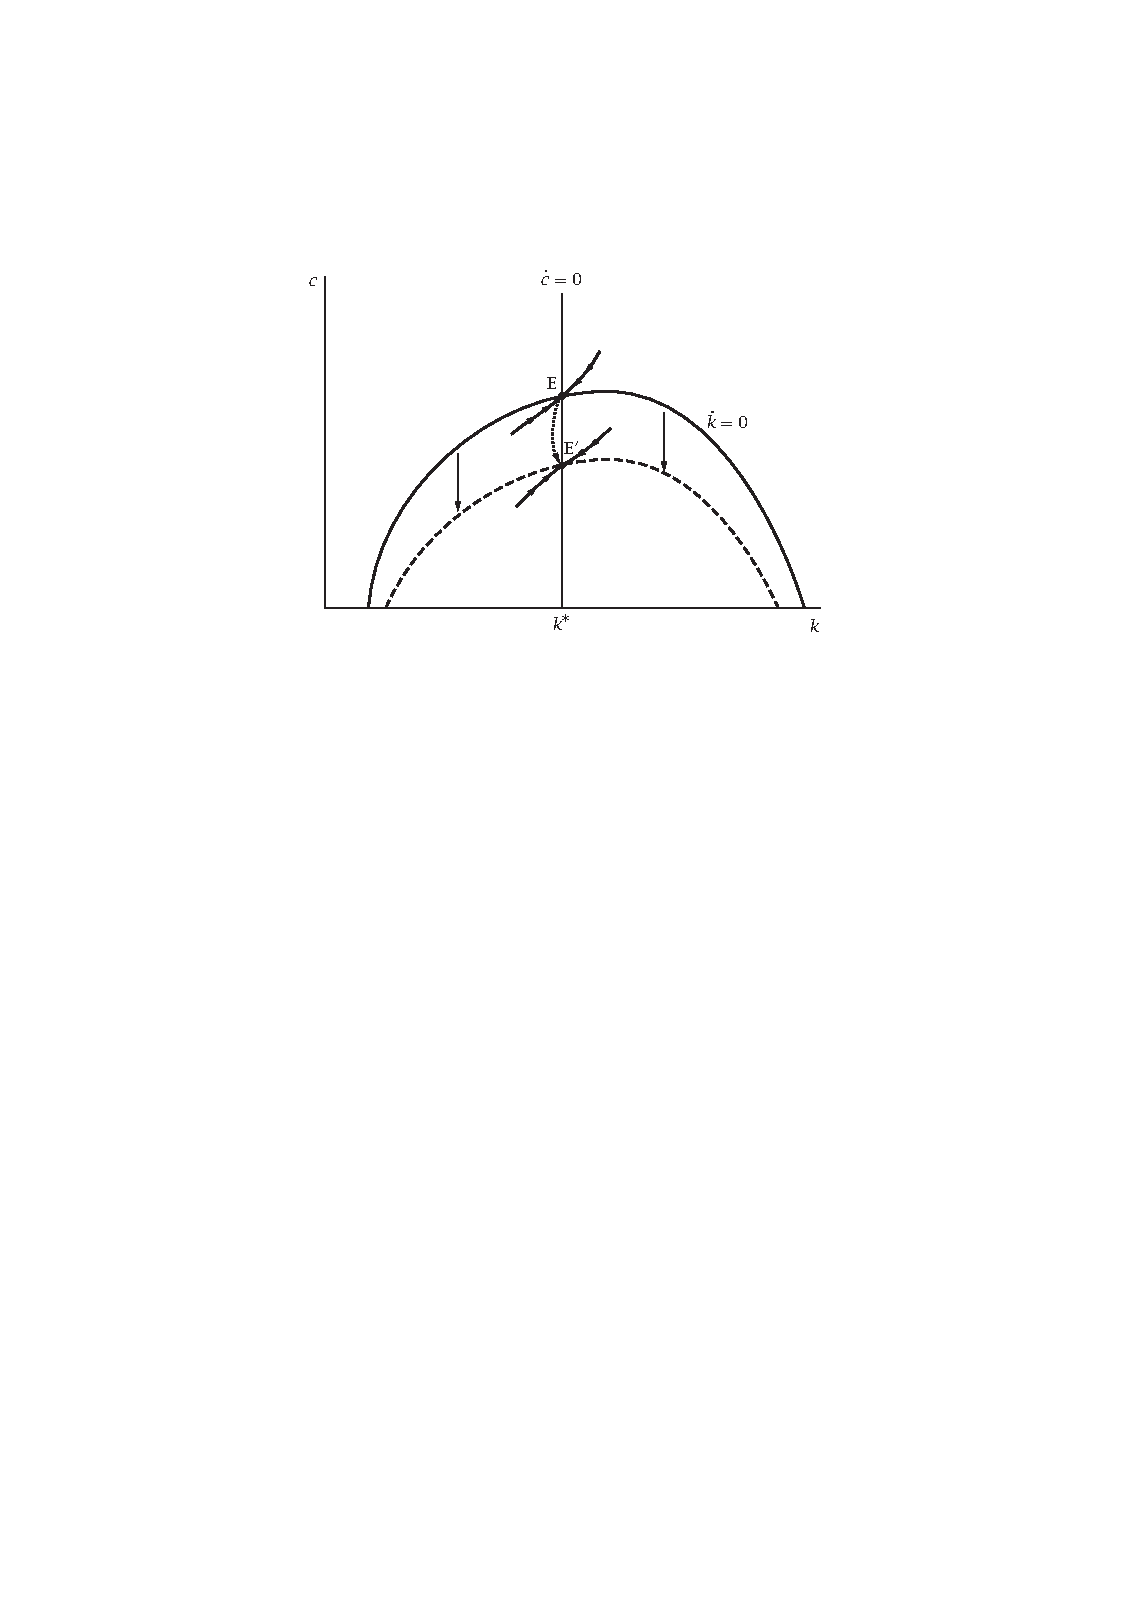
\includegraphics[max width=\linewidth]{1_0_Growth_Theory/RamseyGov.pdf}
    \caption{Government in the Ramsey Model. Source: \textcite{romer_advanced_2012}}  
\end{figure}


Graphically we can see that government expenditure will push the capital accumulation path down, creating a new equilibrium path with lower consumption for the same levels of capital per worker. This is a total crowding out of fiscal policy in a Ramsey Model, because Ricardian Equivalence holds.

\clearpage

\subsection*{Dynamic inefficiency in the Ramsey Model}
As opposed to the Solow model, decisions of savings and consumption in the Ramsey Model is endogenous. Actors will therefore be able to alter their savings and consumption to maximize utility and a dynamic efficiency such as the one we saw in the Solow Model can not exist in the Ramsey Model. The conclusion is slightly different in the OLG-model, mainly because of the assumptions. 

This makes sense given the model's assumptions. If agents are rational, on an infinite time horizon hypothesis, The Ricardian Equivalence\footnote{The Ricardian equivalence proposition is an economic hypothesis holding that consumers are forward looking and so internalize the government's budget constraint when making their consumption decisions. This leads to the result that, for a given pattern of government spending, the method of financing that spending does not affect agents' consumption decisions, and thus, it does not change aggregate demand. Thus, this theorem is used as an argument against tax cuts aimed to boost aggregate demand.} theorem holds, meaning that agents know that any increase in government spending will be need to be financed through future taxes.


\subsubsection{Primary conclusions of the Ramsey Model}
\begin{enumerate}[i]
  \item The steady state is similar to the Solow Model
  \item Saving and consumption decisions are endogenous, and dynamic inefficiency can not exist, because agents are maximizing their utility at any given time given the expectations of the future. 
  \item Countries with higher taxes on investment will have a lower capital stock, lower capital per worker, and lower capital output ratio.
\end{enumerate}